\documentclass[tikz,border=10pt]{standalone}
\usepackage{tkz-graph}
\usepackage{amsmath,amssymb}
\usepackage{xcolor}
\usetikzlibrary{calc}
\usetikzlibrary{positioning, quotes}
\usetikzlibrary{arrows.meta}

\begin{document}


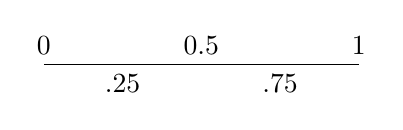
\begin{tikzpicture}
	\draw (0,0) -- node[above, pos=0] {0} node[above, pos=.5] {0.5} node[above, pos=1] {1}
	node[below, pos=.25] {.25}
	node[below, pos=.75] {.75} (4,0);
\end{tikzpicture}



\begin{tikzpicture}[every node/.style = {inner sep=0pt}]
	\node (E) {E};
	\node (p) [base right= 0pt of E] {p};
	\node (i) [base right= 0pt of p] {i};
	\node (c) [base right= 0pt of i] {c};
	\node (.1) [base right= 0pt of c] {.};
\end{tikzpicture}



\begin{tikzpicture}[every pin/.style = {scale=0.5}]
	\node[
		pin = above:Graphics,
		pin = left:Design,
		pin = below:Typography,
		pin = right:Coding,
		circle, shading=ball, ball color=blue!60,
		text=white] {TikZ};
\end{tikzpicture}



\begin{tikzpicture}
	\node [fill=orange, text=white] (tex) {TEX};
	\node [fill={rgb:red,244;green,15;blue,2}, text=white, right = of tex] (pdf)  {PDF};
	\draw (tex) edge[very thick, draw=red, -{Stealth[color=orange, fill=red, width=8pt, length=10pt]}] (pdf);
\end{tikzpicture}


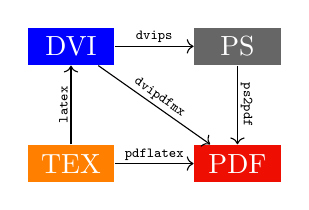
\begin{tikzpicture}[
		every node/.style = {text=white, minimum width =1.1cm},
		every edge/.style = {draw, ->},
		every edge quotes/.style = {text=black, auto, font=\ttfamily\tiny, inner sep=1pt, sloped}]
	\node (tex) [fill=orange] {TEX};
	\node (pdf) [fill={rgb:red,244;green,15;blue,2}, right = of tex] {PDF};
	\node (dvi)  [fill=blue, above= of tex] {DVI};
	\node (ps) [fill=black!60, above = of pdf] {PS};

	\draw (tex) edge["pdflatex"] (pdf);
	\draw (tex) edge["latex"]    (dvi);
	\draw (dvi) edge["dvips"]     (ps);
	\draw (ps)  edge["ps2pdf"]   (pdf);
	\draw (dvi) edge["dvipdfmx"] (pdf);
\end{tikzpicture}

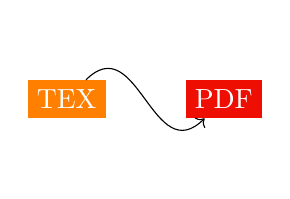
\begin{tikzpicture}
	\node [fill=orange, text=white] (tex) {TEX};
	\node [fill={rgb:red,244;green,15;blue,2}, text=white, right = of tex] (pdf)  {PDF};
	\draw (tex) edge[out=45, in=225, looseness=1.5, ->] (pdf);
\end{tikzpicture}

\end{document}
